%%
%% Beginning of file 'sample.tex'
%%
%% Modified 2015 December
%%
%% This is a sample manuscript marked up using the
%% AASTeX v6.x LaTeX 2e macros.

%% AASTeX is now based on Alexey Vikhlinin's emulateapj.cls 
%% (Copyright 2000-2015).  See the classfile for details.
%%
%% AASTeX requires revtex4-1.cls (http://publish.aps.org/revtex4/) and
%% other external packages (latexsym, graphicx, amssymb, longtable, and epsf).
%% All of these external packages should already be present in the modern TeX 
%% distributions.  If not they can also be obtained at www.ctan.org.

%% The first piece of markup in an AASTeX v6.x document is the \documentclass
%% command. LaTeX will ignore any data that comes before this command. The 
%% documentclass can take an optional argument to modify the output style.
%% The command below calls the preprint style  which will produce a tightly 
%% typeset, one-column, single-spaced document.  It is the default and thus
%% does not need to be explicitly stated.
%%

%% using aastex version 6
\documentclass[twocolumn]{aastex6}

%% The other main article choice is a tightly typeset, two-column article
%% that more closely resembles the final typeset pdf article.
%%
%% \documentclass[twocolumn]{aastex6}
%% 
%% There are other optional arguments one can envoke to allow other 
%% actions. 
%%
% These are the available options:
%   manuscript	: onecolumn, doublespace, 12pt fonts
%   preprint	: onecolumn, single space, 10pt fonts
%   preprint2	: twocolumn, single space, 10pt fonts
%   twocolumn	: a two column article. Probably not needed, but here just in case.
%   onecolumn	: a one column article; default option.
%   twocolappendix: make 2 column appendix
%   onecolappendix: make 1 column appendix is the default. 
%   astrosymb	: Loads Astrosymb font and define \astrocommands. 
%   tighten	: Makes baselineskip slightly smaller
%   times	: uses times font instead of the default
%   linenumbers	: turn on lineno package.
%   trackchanges : required to see the revision mark up and print output
%   numberedappendix: Labels appendix sections A, B, ... This is the default.
%   appendixfloats: Needed. Resets figure and table counters to zero

%% these can be used in any combination, e.g.
%%
%% \documentclass[twocolumn,twocolappendix,linenumbers,trackchanges]{aastex6}

%% If you want to create your own macros, you can do so
%% using \newcommand. Your macros should appear before
%% the \begin{document} command.
%%
\newcommand{\vdag}{(v)^\dagger}
\newcommand\aastex{AAS\TeX}
\newcommand\latex{La\TeX}

%% AASTeX 6.0 supports the ability to suppress the names and affiliations
%% of some authors and displaying them under a "collaboration" banner to
%% minimize the amount of author information that to be printed.  This 
%% should be reserved for articles with an extreme number of authors.
%%
%% Mark up commands to limit the number of authors on the front page.
\AuthorCallLimit=1
%% Will only show Schwarz & Muench since Schwarz and Muench
%% are in the same \author call. 
\fullcollaborationName{The Friends of AASTeX Collaboration}
%% will print the collaboration text after the shortened author list.
%% These commands have to COME BEFORE the \author calls.
%%
%% Note that all of these author will be shown in the published article.
%% This feature is meant to be used prior to acceptance to make the
%% front end of a long author article more manageable.
%% Use \allauthors at the manuscript end to show the full author list.

%% The following command can be used to set the latex table counters.  It
%% is needed in this document because it uses a mix of latex tabular and
%% AASTeX deluxetables.  In general it should not be needed.
%\setcounter{table}{1}

%%%%%%%%%%%%%%%%%%%%%%%%%%%%%%%%%%%%%%%%%%%%%%%%%%%%%%%%%%%%%%%%%%%%%%%%%%%%%%%%
%%
%% The following commented section outlines numerous optional output that
%% can be displayed in the front matter or as running meta-data.
%%
%% You can insert a short comment on the title page using the command below.
%% \slugcomment{Not to appear in Nonlearned J., 45.}
%%
%% If you wish, you may supply running head information, although
%% this information may be modified by the editorial offices.
%%\shorttitle{\aastex sample article}
%%\shortauthors{Schwarz et al.}
%%
%% You can add a light gray and diagonal water-mark to the first page 
%% with this command:
%% \watermark{text}
%% where "text", e.g. DRAFT, is the text to appear.  If the text is 
%% long you can control the water-mark size with:
%% \setwatermarkfontsize{dimension}
%% where dimension is any recognized LaTeX dimension, e.g. pt, in, etc.
%%
%%%%%%%%%%%%%%%%%%%%%%%%%%%%%%%%%%%%%%%%%%%%%%%%%%%%%%%%%%%%%%%%%%%%%%%%%%%%%%%%

%% This is the end of the preamble.  Indicate the beginning of the
%% paper itself with \begin{document}.

\begin{document}

%% LaTeX will automatically break titles if they run longer than
%% one line. However, you may use \\ to force a line break if
%% you desire.

\title{HW 02: Literature Assessment and Measurement and Statistics Practice}

%% Use \author, \affil, plus the \and command to format author and affiliation 
%% information.  If done correctly the peer review system will be able to
%% automatically put the author and affiliation information from the manuscript
%% and save the corresponding author the trouble of entering it by hand.
%%
%% The \affil should be used to document primary affiliations and the
%% \altaffil should be used for secondary affiliations, titles, or email.

%% Authors with the same affiliation can be grouped in a single
%% \author and \affil call.
\author{Bryan Yamashiro\altaffilmark{1}}
\affil{University of Hawaii at Manoa \\
2500 Campus Road \\
Honolulu, HI 96822}


%% Use the \and command so offset the last author.

%% Notice that each of these authors has alternate affiliations, which
%% are identified by the \altaffilmark after each name.  Specify alternate
%% affiliation information with \altaffiltext, with one command per each
%% affiliation.

\altaffiltext{1}{A cool dude}
\altaffiltext{2}{Another cool dude}


%% From the front matter, we move on to the body of the paper.
%% Sections are demarcated by \section and \subsection, respectively.
%% Observe the use of the LaTeX \label
%% command after the \subsection to give a symbolic KEY to the
%% subsection for cross-referencing in a \ref command.
%% You can use LaTeX's \ref and \label commands to keep track of
%% cross-references to sections, equations, tables, and figures.
%% That way, if you change the order of any elements, LaTeX will
%% automatically renumber them.

%% We recommend that authors also use the natbib \citep
%% and \citet commands to identify citations.  The citations are
%% tied to the reference list via symbolic KEYs. The KEY corresponds
%% to the KEY in the \bibitem in the reference list below. 
\section{A Variability Study of Pre-Main Sequence Stars in the Extremely Young Cluster IC 348}
\subsection{Control of Syntax and Mechanics (4/4)}
The paper was generally easy to read, statements were clear and reinforced by literature.
\subsection{Discipline Conventions (4/4)}
Figures, tables, units were well used and standardized. The paper did well to cite specialized proceedings and acronyms.
\subsection{Content (4/4)}
The author used literature well, citing previous work in the field. Citations were also used to previous models that were compared, which showed the importance of the paper to current theory.
\subsection{Reasoning (4/4)}
Approaches were clearly explained, and the procedures to do calculations were included in equations or in cited literature.


\section{Observations and Procedure} \label{sec:intro}


\subsection{Independent Measurements}
The sample size included three individuals of variable wing spans and heights. The instruments used to measure heights utilized a 200\,cm stick, a book, and two wooden blocks. Heights were measured initially by directing the subject to stand flushed against a straight wall. The book was then used as a straight edge to flatten extra height, added by hair, and the perpendicular intersection of the book and wall was marked. Wing span was measured with the subject on the floor. Tiles were measured at (30.5$\pm$0.1)\,cm and used as a full unit, N. The wooden blocks were again used as straight edges and placed to allow for the subject's fingers to be on the edge of a unit. The subject then aligned his/her wingspan along a straight line formed by the tiles and the full wing span was then measured by placing the second block where the wing span ended. Full measurements of wing span, in equation\,\ref{wingspan}, were initiated by adding up the full units first. Then the 200\,cm meter stick was used to measure the fractioned final unit, R, which was then added to the full unit. The three samples are represented in figure\,\ref{bryan}. It is noted that 

\begin{equation}
WS = 30.5N + R
\label{wingspan}
\end{equation}

\begin{figure}[h]
  \centering
    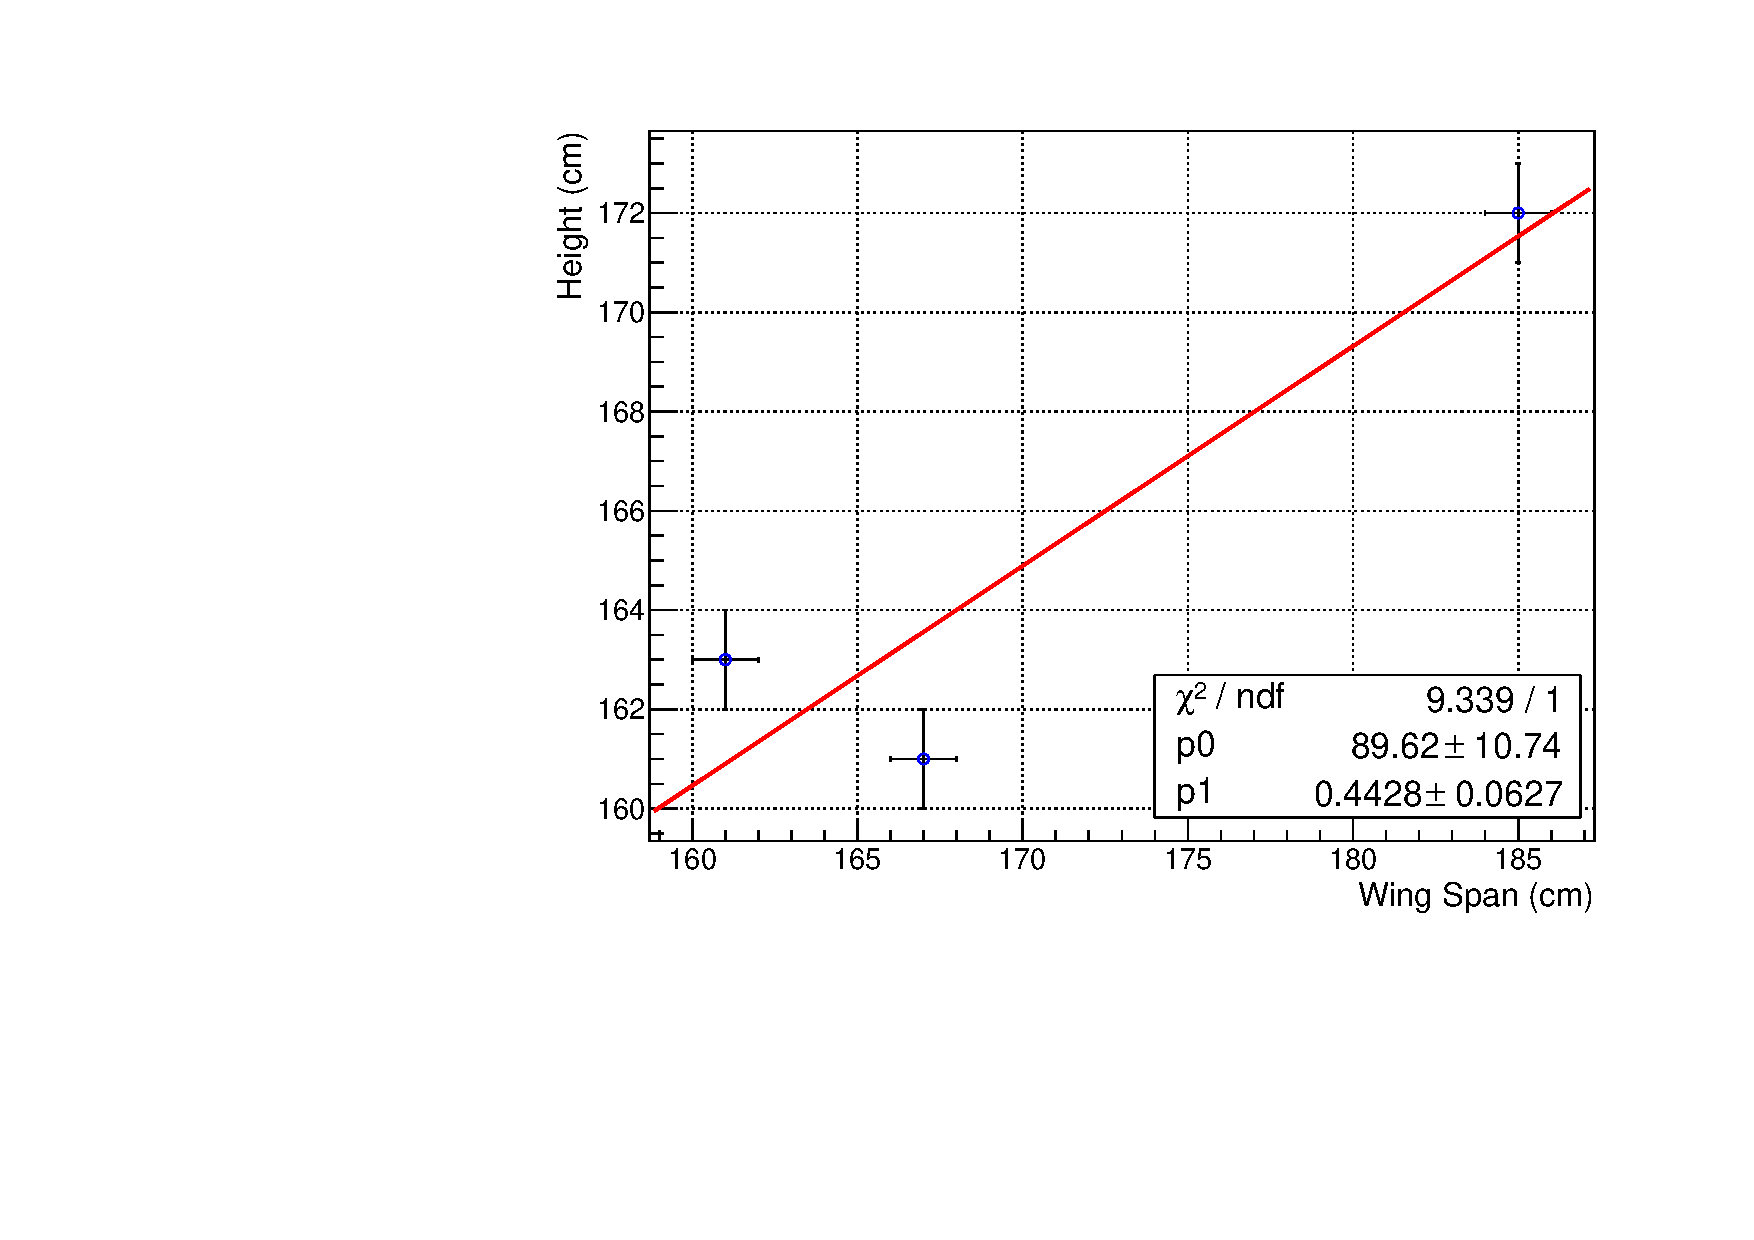
\includegraphics[width=0.5\textwidth]{bry.pdf}
      \caption{Three samples that measured height and wing span derived from the initial procedures. A linear least squares fit was utilized, represented with a red line.}
      \label{bryan}
\end{figure}

\begin{table}[h]
\begin{center}
\caption{Statistics of independent measurements.}

\begin{tabular}{ c|c|c }

Statistics & Height\,(cm)  & Wing Span\,(cm)\\ \hline \hline
Range & 10.5$\pm$0.5 & 23.9$\pm$0.5 \\
 Mean & 165.3$\pm$3.0 & 171.2$\pm$6.9 \\ 
 Median & 1.62.5$\pm$1.0 & 167.3$\pm$1.0 \\  
 Variance & 5.7$\pm$1.0 & 12.4$\pm$1.0 \\

\end{tabular}
\label{indtable}
\end{center}
\end{table}


\clearpage
\subsection{Class Measurements}
The larger sample size consisted of 7 different procedures of measuring height and wing span. The 7 procedure groups resulted in 33 unique measurements. In the class sample, the wing span parameters are generally longer than the heights. Conversely, some samples exhibited longer heights than wing spans.

\begin{figure}[h]
  \centering
    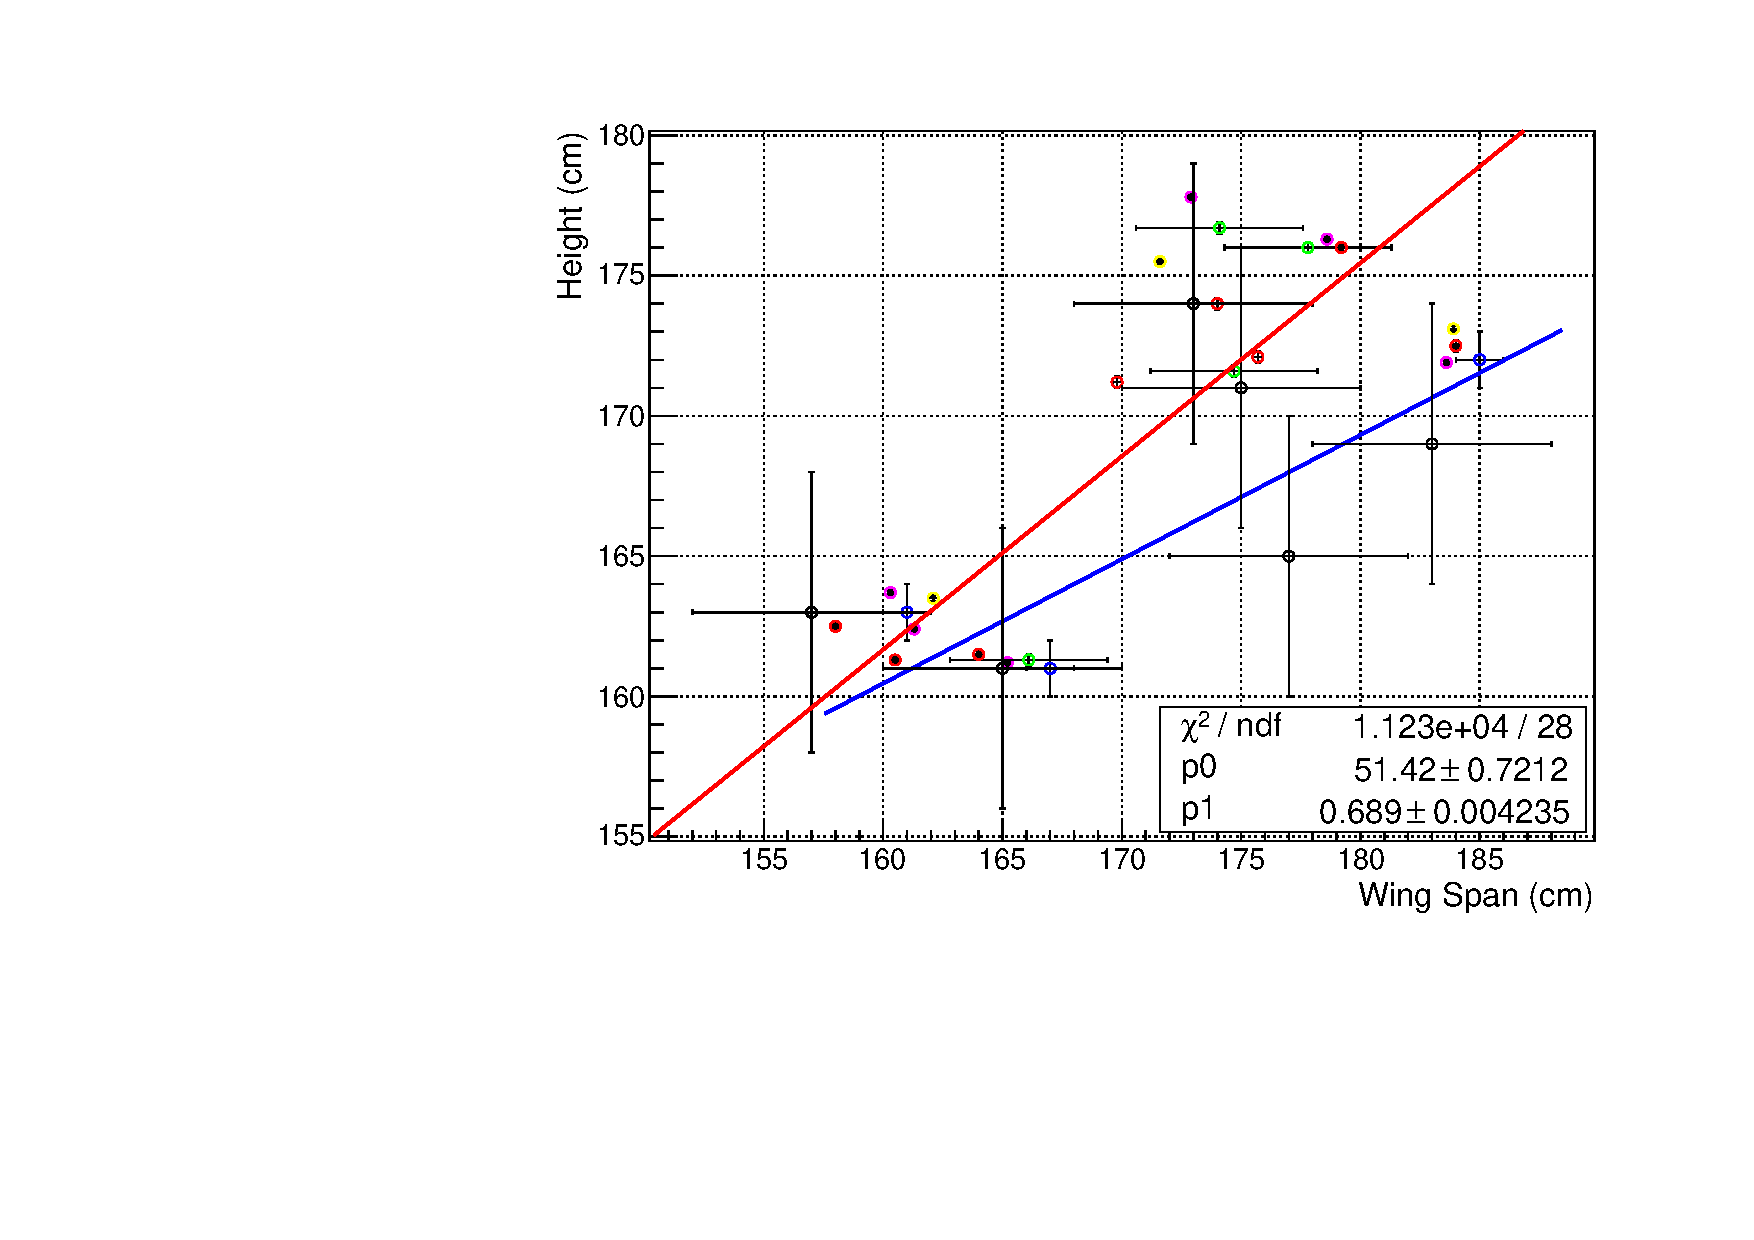
\includegraphics[width=0.5\textwidth]{doublecorr.pdf}
      \caption{The entire class sample of height and wing span measurements that incorporated a variety of procedures. A red least squares fit line is used against the sample data. The blue line corresponds to the fit in figure\,\ref{bryan} for comparative purposes. Different circle colors represent different samples that used variant procedures of measurement. }
      \label{class}
\end{figure}

\begin{table}[b]
\begin{center}
\caption{Statistics of the entire class sample.}

\begin{tabular}{ c|c|c }

Statistics & Height\,(cm)  & Wing Span\,(cm)\\ \hline \hline
Range & 16.8$\pm$4.9 & 30.6$\pm$4.9 \\
 Mean & 169.1$\pm$1.5 & 172.5$\pm$2.7 \\ 
 Median & 171.2$\pm$0.2 & 174.0$\pm$0.2 \\  
 Variance & 5.9$\pm$1.9 & 9.0$\pm$2.0 \\

\end{tabular}
\label{classtable}
\end{center}
\end{table}



\hfill\eject
\section{Discussion}
Both sets of samples show a trend of increased wing span with increasing height measurements. Statistics for both the independent and class measurements are listed in tables\,\ref{indtable} and \ref{classtable}. Comparing the independent sample against the class sample, the class sample accrued a larger mean for both height and wing span. The means of the independent sample for height and wing span were 163$\pm$3.0 and 171.2$\pm$6.9, respectively. These two parameters were compared to the class samples of 169.1$\pm$1.5 and 172.5$\pm$2.7, for height and wing span. Figure\,\ref{class} shows linear least square fits of both data sets. The trends don't exactly measure up, which is most likely due to the tallest students being unmeasured in the independent sample. According to the fits, any individual could have his/her wing span (or height) measured and have the opposing parameter predicted. The class sample shows that in the large spectrum of students at UH Manoa, the height and wing span should be proportional.
\\
\indent The largest source of error is extrapolated from the measurements, as the black circles exhibit over 5\,cm of error in both height and wing span. Systematic error was added mainly for the measuring stick\,(the nearest centimeter was considered) and the straight edge book\,(accounted for the book not being perfectly straight and/or perpendicular to the wall).


%\acknowledgments



\vspace{5mm}

\begin{thebibliography}{}

\bibitem[Audard(2014)]{2}
Chromey, Frederick R. To Measure the Sky: An Introduction to Observational Astronomy. Cambridge: Cambridge UP, 2011. Print.

\bibitem[Herbst(2000)]{1}
Herbst, W., Maley, J. A., \& Williams, E. C. 2000a, AJ, 120, 349

\clearpage

\end{thebibliography}



%% Appendix material should be preceded with a single \appendix command.
%% There should be a \section command for each appendix. Mark appendix
%% subsections with the same markup you use in the main body of the paper.

%% Each Appendix (indicated with \section) will be lettered A, B, C, etc.
%% The equation counter will reset when it encounters the \appendix
%% command and will number appendix equations (A1), (A2), etc.


%% The reference list follows the main body and any appendices.
%% Use LaTeX's thebibliography environment to mark up your reference list.
%% Note \begin{thebibliography} is followed by an empty set of
%% curly braces.  If you forget this, LaTeX will generate the error
%% "Perhaps a missing \item?".
%%
%% thebibliography produces citations in the text using \bibitem-\cite
%% cross-referencing. Each reference is preceded by a
%% \bibitem command that defines in curly braces the KEY that corresponds
%% to the KEY in the \cite commands (see the first section above).
%% Make sure that you provide a unique KEY for every \bibitem or else the
%% paper will not LaTeX. The square brackets should contain
%% the citation text that LaTeX will insert in
%% place of the \cite commands.

%% We have used macros to produce journal name abbreviations.
%% \aastex provides a number of these for the more frequently-cited journals.
%% See the Author Guide for a list of them.

%% Note that the style of the \bibitem labels (in []) is slightly
%% different from previous examples.  The natbib system solves a host
%% of citation expression problems, but it is necessary to clearly
%% delimit the year from the author name used in the citation.
%% See the natbib documentation for more details and options.


\end{document}

%% End of file `sample.tex'.
